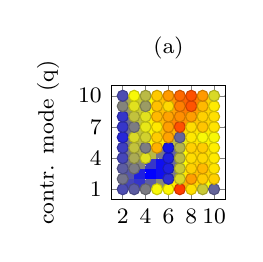
\begin{tikzpicture}
\begin{axis}
[
width=0.25\textwidth,
height=0.25\textwidth,
style={font=\footnotesize},
grid=major,
grid style={dotted},
align=center,
%xlabel={tensor order},
ylabel={contr. mode (q)},
title={{(a)}}, %  ompfor<slice>, asymmetric, row-major
scaled ticks=false,
zlabel={GFlops/core},
view={0}{90}, 
%view={-45}{45}, 
ytick={1,4,7,10},
xtick={2,4,6,8,10},
xmin=1, xmax=11,
ymin=0, ymax=11,
try min ticks=8,
zmin=10, zmax=50,
point meta min=10, point meta max=50,
colormap/hot, 
samples=50,
]
\addplot3[contour filled={number=100},scatter,shader=flat,samples=50]
coordinates{

(2.000,1.000,14.177) (2.000,2.000,16.358) (2.000,3.000,14.869) (2.000,4.000,13.784) (2.000,5.000,13.218) (2.000,6.000,12.389) (2.000,7.000,12.811) (2.000,8.000,13.152) (2.000,9.000,17.167) (2.000,10.000,14.058) 

(3.000,1.000,14.928) (3.000,2.000,1.784) (3.000,3.000,16.681) (3.000,4.000,18.809) (3.000,5.000,20.087) (3.000,6.000,21.317) (3.000,7.000,16.786) (3.000,8.000,20.171) (3.000,9.000,21.800) (3.000,10.000,22.919) 

(4.000,1.000,16.621) (4.000,2.000,3.476) (4.000,3.000,3.324) (4.000,4.000,21.715) (4.000,5.000,16.734) (4.000,6.000,20.909) (4.000,7.000,22.252) (4.000,8.000,21.890) (4.000,9.000,18.106) (4.000,10.000,19.650) 

(5.000,1.000,23.063) (5.000,2.000,6.656) (5.000,3.000,6.354) (5.000,4.000,6.245) (5.000,5.000,31.276) (5.000,6.000,28.747) (5.000,7.000,25.870) (5.000,8.000,30.670) (5.000,9.000,29.994) (5.000,10.000,28.934) 

(6.000,1.000,24.099) (6.000,2.000,12.542) (6.000,3.000,11.879) (6.000,4.000,11.622) (6.000,5.000,11.371) (6.000,6.000,33.174) (6.000,7.000,33.505) (6.000,8.000,33.144) (6.000,9.000,27.321) (6.000,10.000,33.741) 

(7.000,1.000,43.545) (7.000,2.000,21.351) (7.000,3.000,20.534) (7.000,4.000,19.951) (7.000,5.000,19.439) (7.000,6.000,15.298) (7.000,7.000,41.259) (7.000,8.000,35.160) (7.000,9.000,36.637) (7.000,10.000,38.996) 

(8.000,1.000,26.764) (8.000,2.000,33.491) (8.000,3.000,28.294) (8.000,4.000,26.895) (8.000,5.000,28.272) (8.000,6.000,25.903) (8.000,7.000,26.818) (8.000,8.000,33.547) (8.000,9.000,40.813) (8.000,10.000,41.255) 

(9.000,1.000,20.798) (9.000,2.000,28.583) (9.000,3.000,30.483) (9.000,4.000,27.264) (9.000,5.000,28.433) (9.000,6.000,22.847) (9.000,7.000,29.367) (9.000,8.000,28.364) (9.000,9.000,30.574) (9.000,10.000,33.672) 

(10.000,1.000,15.559) (10.000,2.000,28.090) (10.000,3.000,26.263) (10.000,4.000,25.477) (10.000,5.000,24.815) (10.000,6.000,22.805) (10.000,7.000,26.381) (10.000,8.000,26.505) (10.000,9.000,25.500) (10.000,10.000,21.425) 

};
\end{axis}
\end{tikzpicture}
\hfill
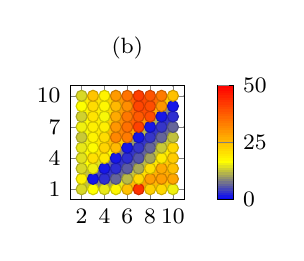
\begin{tikzpicture}
\begin{axis}
[
width=0.25\textwidth,
height=0.25\textwidth,
style={font=\footnotesize},
grid=major,
grid style={dotted},
align=center,
%xlabel={tensor order},
%ylabel={contr. mode (q)},
title={{(b)}}, %  ompfor<subtensor>, asymmetric, row-major
scaled ticks=false,
zlabel={GFlops},
view={0}{90}, 
ytick={1,4,7,10},
xtick={2,4,6,8,10},
xmin=1, xmax=11,
ymin=0, ymax=11,
try min ticks=8,
zmin=0, zmax=50,
point meta min=0, point meta max=50,
colormap/hot, 
samples=50,
colorbar sampled,
colorbar/width=0.2cm,
colorbar style={
point meta min=0, point meta max=50,
samples=50,
font=\footnotesize,
ytick={0,25,50},
yticklabels={0,25,50},
%title={\scriptsize Gflops},
%ylabel={\scriptsize Gflops},
}
]
\addplot3[contour filled={number=100},scatter,shader=flat,samples=50]
coordinates{

(2.000,1.000,14.150) (2.000,2.000,18.168) (2.000,3.000,14.380) (2.000,4.000,14.818) (2.000,5.000,15.416) (2.000,6.000,13.081) (2.000,7.000,15.551) (2.000,8.000,13.981) (2.000,9.000,16.961) (2.000,10.000,14.297) 

(3.000,1.000,16.658) (3.000,2.000,1.780) (3.000,3.000,15.940) (3.000,4.000,20.908) (3.000,5.000,17.001) (3.000,6.000,18.151) (3.000,7.000,18.853) (3.000,8.000,20.356) (3.000,9.000,21.150) (3.000,10.000,24.034) 

(4.000,1.000,15.470) (4.000,2.000,3.473) (4.000,3.000,1.763) (4.000,4.000,19.978) (4.000,5.000,22.019) (4.000,6.000,21.370) (4.000,7.000,18.694) (4.000,8.000,16.418) (4.000,9.000,17.892) (4.000,10.000,18.183) 

(5.000,1.000,17.885) (5.000,2.000,6.625) (5.000,3.000,3.373) (5.000,4.000,1.701) (5.000,5.000,25.808) (5.000,6.000,32.283) (5.000,7.000,30.427) (5.000,8.000,27.599) (5.000,9.000,25.759) (5.000,10.000,29.893) 

(6.000,1.000,24.716) (6.000,2.000,12.440) (6.000,3.000,6.321) (6.000,4.000,3.193) (6.000,5.000,1.782) (6.000,6.000,33.517) (6.000,7.000,35.466) (6.000,8.000,34.242) (6.000,9.000,31.231) (6.000,10.000,34.605) 

(7.000,1.000,43.408) (7.000,2.000,21.521) (7.000,3.000,11.123) (7.000,4.000,5.561) (7.000,5.000,3.508) (7.000,6.000,1.784) (7.000,7.000,41.398) (7.000,8.000,38.079) (7.000,9.000,40.652) (7.000,10.000,41.770) 

(8.000,1.000,22.875) (8.000,2.000,29.491) (8.000,3.000,20.653) (8.000,4.000,10.787) (8.000,5.000,6.814) (8.000,6.000,3.511) (8.000,7.000,1.788) (8.000,8.000,39.967) (8.000,9.000,39.718) (8.000,10.000,38.518) 

(9.000,1.000,21.665) (9.000,2.000,29.387) (9.000,3.000,27.538) (9.000,4.000,19.369) (9.000,5.000,13.041) (9.000,6.000,6.810) (9.000,7.000,3.504) (9.000,8.000,1.769) (9.000,9.000,30.494) (9.000,10.000,33.784) 

(10.000,1.000,15.677) (10.000,2.000,28.056) (10.000,3.000,24.845) (10.000,4.000,23.423) (10.000,5.000,21.554) (10.000,6.000,12.533) (10.000,7.000,6.784) (10.000,8.000,3.476) (10.000,9.000,1.758) (10.000,10.000,24.585) 


};
\end{axis}
\end{tikzpicture}
\hfill
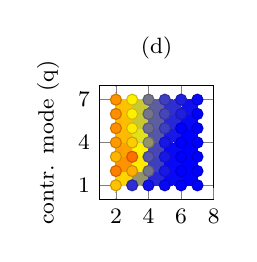
\begin{tikzpicture}
\begin{axis}
[
width=0.25\textwidth,
height=0.25\textwidth,
style={font=\footnotesize},
grid=major,
grid style={dotted},
align=center,
%xlabel={tensor order},
ylabel={contr. mode (q)},
title={{(d)}}, %  ompfor<slice>, symmetric, row-major
scaled ticks=false,
zlabel={GFlops},
view={0}{90}, 
ytick={1,4,7,10},
xtick={2,4,6,8},
xmin=1, xmax=8,
ymin=0, ymax=8,
try min ticks=8,
zmin=0, zmax=55,
point meta min=0, point meta max=55,
colormap/hot, 
samples=50,
]
\addplot3[contour filled={number=100},scatter,shader=flat,samples=50]
coordinates{

(2.000,1.000,27.090) (2.000,2.000,36.633) (2.000,3.000,28.737) (2.000,4.000,32.791) (2.000,5.000,34.606) (2.000,6.000,34.332) (2.000,7.000,33.607) 

(3.000,1.000,3.535) (3.000,2.000,30.198) (3.000,3.000,38.963) (3.000,4.000,25.423) (3.000,5.000,21.062) (3.000,6.000,20.381) (3.000,7.000,20.382) 

(4.000,1.000,1.243) (4.000,2.000,8.485) (4.000,3.000,6.219) (4.000,4.000,10.477) (4.000,5.000,8.056) (4.000,6.000,8.354) (4.000,7.000,8.337) 

(5.000,1.000,0.702) (5.000,2.000,1.700) (5.000,3.000,1.650) (5.000,4.000,1.662) (5.000,5.000,4.782) (5.000,6.000,5.217) (5.000,7.000,4.731) 

(6.000,1.000,0.391) (6.000,2.000,0.218) (6.000,3.000,0.219) (6.000,4.000,0.219) (6.000,5.000,0.220) (6.000,6.000,2.476) (6.000,7.000,2.653) 

(7.000,1.000,0.307) (7.000,2.000,0.026) (7.000,3.000,0.027) (7.000,4.000,0.027) (7.000,5.000,0.027) (7.000,6.000,0.027) (7.000,7.000,0.839) 


};
\end{axis}
\end{tikzpicture}
\hfill
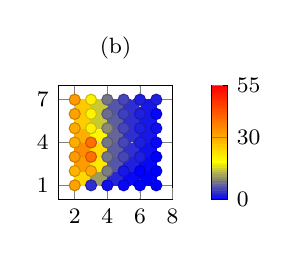
\begin{tikzpicture}
\begin{axis}
[
width=0.25\textwidth,
height=0.25\textwidth,
style={font=\footnotesize},
grid=major,
grid style={dotted},
align=center,
%xlabel={tensor order},
%ylabel={contr. mode (q)},
title={{(b)}}, %  ompfor<subtensor>, symmetric, row-major
scaled ticks=false,
zlabel={GFlops},
view={0}{90}, 
%view={-45}{45}, 
ytick={1,4,7,10},
xtick={2,4,6,8},
xmin=1, xmax=8,
ymin=0, ymax=8,
try min ticks=8,
zmin=0, zmax=55,
point meta min=0, point meta max=55,
colormap/hot, 
samples=50,
colorbar sampled,
colorbar/width=0.2cm,
colorbar style={
point meta min=0, point meta max=55,
samples=50,
font=\footnotesize,
ytick={0,30,55},
yticklabels={0,30,55},
%title={\scriptsize Gflops},
%ylabel={\scriptsize Gflops},
}
]
\addplot3[contour filled={number=100},scatter,shader=flat,samples=50]
coordinates{

(2.000,1.000,31.720) (2.000,2.000,28.835) (2.000,3.000,32.560) (2.000,4.000,29.729) (2.000,5.000,30.367) (2.000,6.000,31.442) (2.000,7.000,32.686) 

(3.000,1.000,3.525) (3.000,2.000,30.655) (3.000,3.000,38.818) (3.000,4.000,38.927) (3.000,5.000,20.463) (3.000,6.000,20.182) (3.000,7.000,20.852) 

(4.000,1.000,1.205) (4.000,2.000,9.073) (4.000,3.000,8.324) (4.000,4.000,8.252) (4.000,5.000,9.954) (4.000,6.000,7.973) (4.000,7.000,8.301) 

(5.000,1.000,0.658) (5.000,2.000,1.760) (5.000,3.000,5.100) (5.000,4.000,5.138) (5.000,5.000,5.269) (5.000,6.000,4.879) (5.000,7.000,4.964) 

(6.000,1.000,0.331) (6.000,2.000,0.219) (6.000,3.000,2.300) (6.000,4.000,2.632) (6.000,5.000,2.349) (6.000,6.000,2.437) (6.000,7.000,2.383) 

(7.000,1.000,0.310) (7.000,2.000,0.026) (7.000,3.000,0.360) (7.000,4.000,0.846) (7.000,5.000,1.135) (7.000,6.000,0.930) (7.000,7.000,2.590) 


};
\end{axis}
\end{tikzpicture}